\section{Vista de Procesos}

En la implementación actual se distinguen tres procesos lógicos principales, desplegados
como servicios independientes:

\begin{itemize}
  \item \textbf{Cliente}: el navegador del usuario, donde se ejecuta la aplicación web. Desde aquí se realizan las peticiones HTTP al sistema, tanto para
        cargar la interfaz inicial como para invocar la API (por ejemplo, login, gestión
        de pedidos, consulta de menú, etc.).
  \item \textbf{Servidor de frontend}: servicio web que sirve los recursos
        estáticos de la aplicación (HTML, CSS, JavaScript) y actúa como punto de entrada
        público. Una vez cargada la app web en el navegador, el servidor de frontend sigue
        atendiendo peticiones de recursos estáticos, pero la mayor parte de la
        interacción ocurre entre el cliente y la API backend.
  \item \textbf{Servidor backend}: aplicación Spring Boot que implementa las capas de
        controlador, servicio y persistencia. Expone la API REST que utiliza el cliente
        para todas las operaciones de negocio (usuarios, autenticación, pedidos, menú,
        descuentos, etc.) y se comunica con la base de datos relacional.
\end{itemize}

Adicionalmente existe un proceso de base de datos (PostgreSQL) que persiste el estado
del sistema y que es utilizado exclusivamente por el servidor backend. En el diagrama
se lo representa como un servicio de soporte para simplificar el foco en la interacción
cliente--aplicación.

\begin{figure}[htbp]
          \centering
          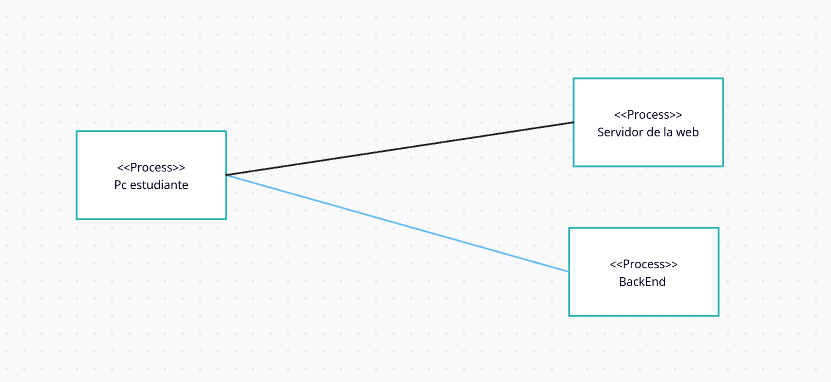
\includegraphics[width=0.9\textwidth]{img/Vista_procesos.png}
          \caption{Diagrama de la vista de procesos}
          \label{fig:mi_imagen}
        \end{figure}

\newpage